\documentclass[dvipsnames, usenames]{beamer}

\usepackage[english]{babel}
\usepackage[utf8]{inputenc}
\usepackage{graphicx}
\usepackage{helvet}
\usepackage{hyperref}

\usetheme{Pittsburgh}
%\usecolortheme{structure}
\usefonttheme{structurebold}

\parskip=1.5ex
\newcommand{\spacepls}{\vspace{1.5Ex}}
\beamertemplatenavigationsymbolsempty
\setbeamersize{description width=0.57cm}

\hypersetup{
	colorlinks=true,
	urlcolor=blue,
	linkcolor=black
	}

\title{The very basics of Git}
\subtitle{\texttt{git} for the non-programmer}

\author[X. Sánchez Díaz]{Xavier~Sánchez Díaz\\\texttt{mail@tec.mx}}
\institute[ITESM]{Research Group with Strategic Focus on Intelligent Systems\\
Tecnológico de Monterrey, Campus Monterrey}
\date{}
\subject{The very basics of Git}

\begin{document}

\begin{frame}
	\titlepage
\end{frame}

\begin{frame}%[allowframebreaks]
	{Outline}
	\tableofcontents
\end{frame}

\section{Preamble} % (fold)
\label{sec:preamble}

\subsection{The UNIX Philosophy} % (fold)
\label{sec:philosophy}

\begin{frame}{Everything is a file}{The UNIX philosophy}

	\spacepls

	\begin{itemize}
		\item Source code is stored in files. \pause
		\item Word documents are files. \pause
		\item Photos are files. \pause
		\item Videos are files. \pause
		\item HDDs and USBs are files. \pause
	\end{itemize}

	\spacepls
	{\huge Everything \pause is \pause a \pause file.}\\
\end{frame}

\begin{frame}{Everything is a file}{The UNIX philosophy}

	\spacepls

	Since everything is a file, it makes sense to keep track of the changes of your projects using \texttt{git}, no matter what you're working on!

	Changes are labeled with a unique identifier, a message and then linked to the user (both name and email) who submitted the modification.
	
	A user can also look and revisit any state of the project throughout its lifetime, and see the differences between two versions of a file at a given state.
	
\end{frame}

% subsection philosophy (end)

\subsection{What is Git?} % (fold)
\label{sub:what_is_git}

\begin{frame}{What is \texttt{git}?}{And why should I use it?}

	\spacepls

	\texttt{git} is a {\color{OliveGreen}free and open source} \alert{distributed} {\color{Blue}version control system}. \pause

	\bigskip

	\begin{block}{Version control system}	
		A system that allows easy management project versions.
	\end{block} \pause

	\bigskip

	\begin{alertblock}{Distributed}	
		Not centralized. Everyone on the team has their own local copy.
	\end{alertblock} \pause

	\bigskip

	\begin{exampleblock}{Free and Open Source}	
		Git is distributed according to a GPLv2 License.
	\end{exampleblock}
	
\end{frame}


\begin{frame}{Free speech, not free beer}{What is \texttt{git}?}

	Git is free software since it respects the four essential freedoms of the user: \pause

	\begin{itemize}
		\item Freedom to use the program as you wish, for any purpose. \pause
		\item Freedom to modify the software as you want. The source code is there for you to look at and modify at will. \pause
		\item Freedom to share or redistribute copies as you wish to help your neighbor. \pause
		\item Freedom to share or redistribute copies of your modified versions to others.
	\end{itemize}
	
\end{frame}

\begin{frame}{What is \texttt{git}?}{And why should I use it?}

	A version control system tracks changes on projects.
	It is a useful tool to keep track of the following: \pause

	\begin{itemize}
		\item What changed since the last version? \pause
		\item When was the last modification? \pause
		\item Who was the last person on the team to modify this file? \pause
		\item Which version is the one I'm looking for? \pause
	\end{itemize}

	So you can avoid having filenames like \texttt{Projectfinal3lastrev18.doc} or \texttt{Projectfinal(this\_is\_the\_one).pdf}.

\end{frame}

% subsection what_is_git (end)

\subsection{\texttt{git} is not GitHub} % (fold)
\label{sub:git-not-github}

\begin{frame}[allowframebreaks]{\texttt{git} is not GitHub}{Let's get it right}

	\begin{figure}[h]
		\centering
		
\includegraphics[width=0.45\textwidth]{logo}
		\label{fig:git-logo}
	\end{figure}

	\textbf{Git} is the software: a technology and a workflow methodology.

	\framebreak

	\begin{figure}[h]
		\centering
		
\includegraphics[width=0.25\textwidth]{octocat}
		\label{fig:github-logo}
	\end{figure}

	\textbf{GitHub} is a website that offers `free' (as in free beer) hosting of open source projects.
	GitHub uses the Git methodology. There are plenty of alternatives to GitHub.
\end{frame}

% subsection git-not-github (end)
% section preamble (end)

\section{The Git workflow}
\subsection{How does Git work?}

\begin{frame}{How does it work?}{The Git workflow}
	Assume you're in charge of a feature. Then, the process would be similar to the following: \pause

	\begin{enumerate}
		\setcounter{enumi}{-1}
		\item<12-> Update your copy to the newest version {\scriptsize on your computer}
		\item<2-> Make some changes \onslide<8->{\alert<8>{\scriptsize to your files}}
		\item<3-> Prepare and stage those changes \onslide<8->{\alert<8>{\scriptsize in your computer}}
		\item<4-> Accept and label the changes \onslide<8->{\alert<8>{\scriptsize in your computer}}
		\item<5-> Submit your labeled changes \onslide<9->{\alert<9>{\scriptsize to the master repository}}
		\item<6-> Your changes are accepted and incorporated to the project \onslide<9->{\alert<9>{\scriptsize on the master repository}}
		\item<7-11> Everyone updates their copy to the newest version \onslide<10-11>{\alert<10>{\scriptsize on their computers}}
	\end{enumerate}
\end{frame}

\subsection{The distributed architecture}

\begin{frame}{What and where?}{The Git workflow}
	\begin{figure}[h]
		\centering
		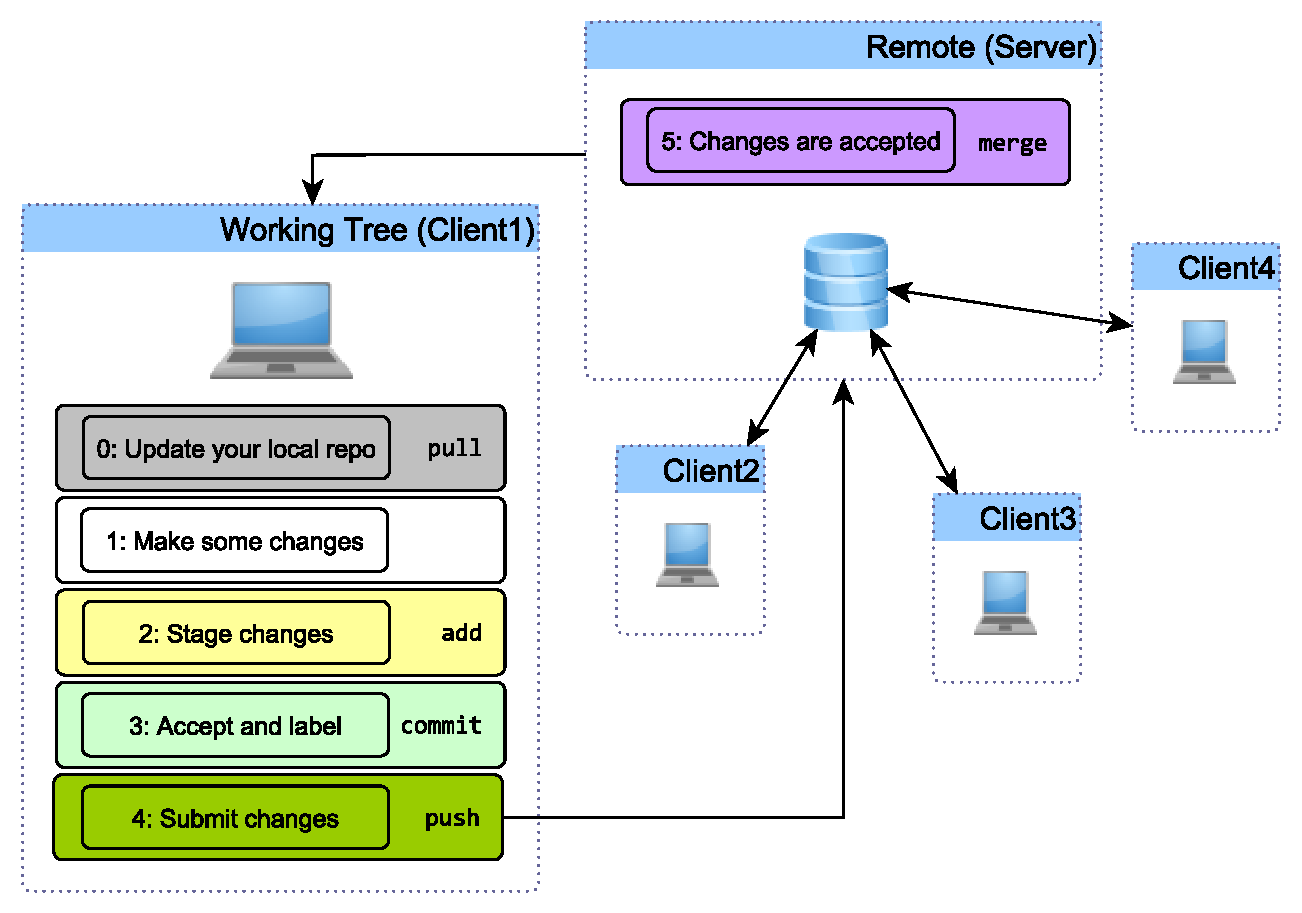
\includegraphics[width=0.97\columnwidth]{stages}
		\label{fig:git-workflow}
	\end{figure}
\end{frame}

\subsection{Branches and merges}

\begin{frame}{Branching}{The Git workflow}
	\begin{figure}[h]
		\centering
		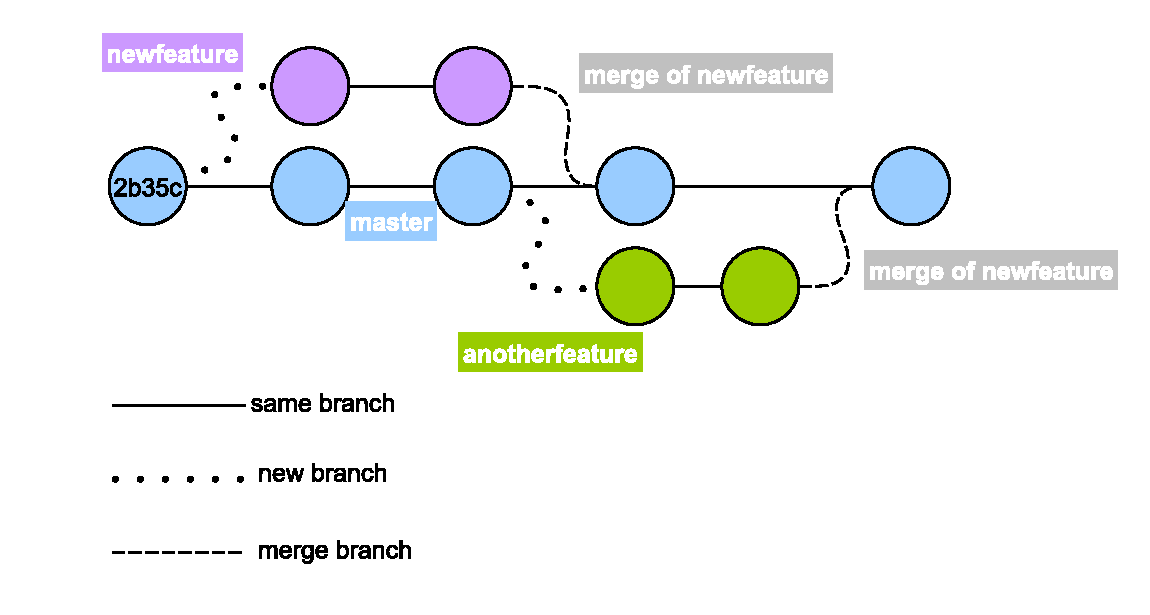
\includegraphics[width=0.97\columnwidth]{branches}
		\label{fig:git-branches}
	\end{figure}
\end{frame}

\subsection{\texttt{git} commands in the shell}

\begin{frame}{\texttt{git} command syntax}{The git workflow}
	Git is usually run in a \textsc{UNIX}-like console. As such, you invoke \alert{commands} like this: \pause

	\begin{center}
		\Large
		\texttt{\$ git <command> [arguments]}
	\end{center} \pause

	The most common commands are \texttt{init}, \texttt{clone}, \texttt{add}, \texttt{commit}, \texttt{push}, \texttt{pull}, \texttt{checkout}, \texttt{branch}, \texttt{log}, \texttt{remote} and \texttt{diff}. \pause

	All commands have different \alert{arguments} (or \textbf{options}). You can check the available options (and the syntax) using the \texttt{--help} option for any of the available commands in git: \pause

	\begin{center}
		\Large
		\texttt{\$ git add --help}
	\end{center}
\end{frame}

\section{Recap}

\begin{frame}{Now with commands!}{Recap}
	\begin{description}
		\item[Update your copy to the newest version] with \texttt{git pull <repository> [branch]}.
		\item[Make some changes] by editing and saving your work. You have some \textbf{unstaged} changes by now.
		\item[Stage those changes] using \texttt{git add <file>}. Your files are now \textbf{staged} and ready to be labeled.
		\item[Label the changes] by using \texttt{git commit [options]}, your work is now \textbf{committed} with a hash (SHA-1) and linked to your user.
		\item[Submit your labeled changes to the master repository] by using \texttt{git push [options]}.
		\item[Your changes are incorporated to the project] by merging the branch you worked on, with \texttt{git merge [options]}. This is usually done by an administrator.
	\end{description}
\end{frame}

\begin{frame}[plain]
	\begin{center}
		{\Huge
		That's it!}

		\bigskip

		{\huge
		For more information
		}

		\bigskip

		Be sure to check out the documentation for \texttt{git} in its \href{https://git-scm.com/}{official webpage}.
		They also have a free book!

		You can also take a look at the \href{https://github.com/}{GitHub}, \href{https://gitlab.com/}{GitLab} and \href{https://bitbucket.org/}{Bitbucket} \texttt{git} tutorials.
	\end{center}
\end{frame}

\end{document}